

\chapter{Wstęp teoretyczny}
	\texttt{Robot mobilny} - robot, który potrafi zmieniać swoje położenie w przestrzeni. Może być robotem autonomicznym, czyli takim który realizując swoje zadanie porusza się bezkolizyjnie w wyznaczonym środowisku oraz robi to bez ingerencji operatora.
	
	Roboty mobilne można podzielić ze względu na ich mobliność:
	\begin{itemize}
		\item kołowe
		\item kroczące
		\item latające
		\item pływające
	\end{itemize}
	Z kolei w robotach kołowych możemy rozróżnić następujące klasy:
	\begin{itemize}
		\item (3,0) - robot posiadający 3 koła szwedzkie. Najczęściej spotykany w formie trójkątnej platformy z przymocowanymi kołami do wierzchołków trójkąta. Jego zaletą jest możliwość poruszania się w dowolnym kierunku. Natomiast wadą trudne sterowanie.
		\item (2,1) - robot posiada 2 koła kastora z tyłu oraz jedno obrotowe, napędowe z przodu. Zaletą jest prostota konstrukcji natomiast wadą trudne sterowanie oraz wrażliwość na nierówności terenu.
		\item (2,0) - robot tzw. unicycle. Posiada 2 niezależnie napędzane koła, ustawione naprzeciwko siebie. Są one przymocowane na sztywno do ramy. Robot ten musi posiadać także punkt podparcia, którym najczęściej jest koło kastora. Plusami takiego rozwiązania jest prostota sterowania oraz konstrukcji. Dodatkowo robot posiada możliwość obrotu w miejscu. Minusem natomiast jest jego wrażliwość na nierówności.
		\item (1,2) - robot posiada 2 koła napędowe, skrętne oraz jedno koło kastora służące za podporę. Konstrukcja wymaga zastosowania 3 silników, 2 do zmiany kąta każdego z kół oraz jeden napędowy. Tak więc minusem takiego rozwiązania jest jego skomplikowane sterowanie
		\item (1,1) - robot nazywany także samochodem kinematycznym ponieważ zachowuje się podczas sterowania jak zwykły samochód. Jego plusem jest niska wrażliwość na nierówności powierzchni, a jego minusem duży promień skrętu.
	\end{itemize}
	
	Jedynym holonomicznym z wyżej wymienionych klas robotów mobilnych kołowym, jest klasa (3,0). \newline \newline \newline
	\textcolor{red}{Holonomiczność} - to w uproszczeniu brak ograniczeń na przeprowadzenie ruchu.
	\newline \newline \newline
	Do sterowania kierunkiem obrotów silnika szczotkowego DC wykorzystuje się układ zwany mostkiem H. Jest on przedstawiony schematycznie na rysunku \ref{fig:mostekHschemat}. 
	
	\begin{figure}[H]
		\centering
		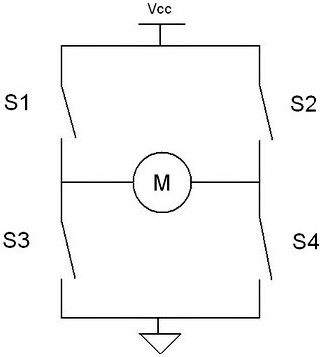
\includegraphics[width=0.4\textwidth]{rys01/mostekH.jpeg} 
		\caption{Schemat mostka H}
		\label{fig:mostekHschemat}
	\end{figure}

	Styki oznaczone literą S i silnik oznaczony literą M przypominają kształt dużej litery H. Jego działanie polega na zwieraniu odpowiednio styków S1 oraz S4 aby uzyskać kierunek obrotów w jedną stronę. Chcąc uzyskać obroty w drugą stronę należy zewrzeć styki S2 i S3. Należy mieć na uwadze odpowiednie sterowanie ponieważ załączenie w jednym czasie styków S1 i S3 lub S2 i S4 spowoduje zwarcie.
%%%
%%%Uwaga: tytuł powinien zmieścić się w okienku kolorowej okładki (którą
%%%powinna dostarczyć uczelniana administracja). Proszę posterować
%%%parametrami, aby "wpasować" w okienko własny tekst.
%%%
%%%Do ASAPa należy wprowadzić pracę dyplomową/projekt inżynierski w pliku o nazwie:
%%%
%%%W04_[nr albumu]_[rok kalendarzowy]_[rodzaj pracy] (szczegółowa instrukcja pod adresem asap.pwr.edu.pl)
%%%
           %%%Przykładowo:
        %%%­W04_123456_2015_praca inżynierska.pdf     - praca dyplomowa inżynierska
        %%%W04_123456_2015_projekt inżynierski.pdf   - projekt inżynierski
        %%%W04_123456_2015_praca magisterska.pdf  - praca dyplomowa magisterska
%%%
              %%%rok kalendarzowy ? rok realizacji kursu „Praca dyplomowa” (nie rok obrony) 